\documentclass[conference,10.6cpt]{IEEEtran}
\ifCLASSINFOpdf \usepackage[pdftex]{graphicx} \else \fi
\usepackage{verbatim}
\usepackage{amsmath}
\usepackage{tipa}
\usepackage{lmodern}
\usepackage{upgreek}
\usepackage{amsfonts}
\usepackage{bm}
\usepackage{bbm, dsfont}
\usepackage{upquote}
\usepackage{mathtools}
\usepackage{algorithmicx}
\usepackage{array}
\usepackage[caption=false,font=normalsize,labelfont=sf,textfont=sf]{subfig}
\usepackage{fixltx2e}
\usepackage{url}
\usepackage{multirow}
\usepackage{caption}
\setlength{\baselineskip}{11pt}
\hyphenation{op-tical net-works semi-conduc-tor}
\newcommand{\bD}{\bm{D}}
\newcommand{\bG}{\bm{G}}
\newcommand{\bI}{\bm{I}}
\newcommand{\bDelta}{\bm{\Delta}}
\newcommand{\oH}{\bm{\overline{H}}}
\newcommand{\ooH}{\bm{\overline{\overline{H}}}}
\newcommand{\hH}{\bm{\hat{H}}}
\newcommand{\hPsi}{\bm{\hat{\Psi}}}
\newcommand{\htheta}{\bm{\hat{\uptheta}}}
\newcommand{\hPhi}{\bm{\hat{\Phi}}}
\newcommand{\tDelta}{\bm{\tilde{\Delta}}}
\newcommand{\tD}{\bm{\tilde{D}}}
\newcommand{\remove}[1]{}
\newcommand{\ie}{i.e.,\ }
\newcommand{\bigie}{I.e.,\ }
\begin{document}

\title{Efficient Implementation of Enhanced Adaptive
  Simultaneous Perturbation Algorithms}
\author{\IEEEauthorblockN{Pushpendre Rastogi}
  \IEEEauthorblockA{Department of Computer Science\\ The Johns Hopkins
    University\\ Baltimore, MD 21218\\ Email: pushpendre@jhu.edu} \and
  \IEEEauthorblockN{Jingyi Zhu} \IEEEauthorblockA{Department of Applied
    Mathematics and Statistics\\ The Johns Hopkins University\\ Baltimore,
    MD 21218\\ Email: jingyi.zhu@jhu.edu} \and \IEEEauthorblockN{James
    C. Spall} \IEEEauthorblockA{Applied Physics Laboratory\\ The Johns
    Hopkins University\\ Laurel, MD 20723\\ Email:
    james.spall@jhuapl.edu}}

\maketitle

\begin{abstract} Stochastic approximation (SA) applies in both the
  gradient-free optimization (Kiefer-Wolfowitz) and the gradient-based
  setting (Robbins-Monro). The idea of simultaneous perturbation (SP) has been well established. This paper discusses an efficient way of
  implementing both the adaptive Newton-like SP algorithms and their enhancements
  (feedback and optimal weighting incorporated), using the Woodbury
  matrix identity, a.k.a. matrix inversion lemma. Basically, instead of
  estimating the Hessian matrix directly, this paper deals with the
  estimation of the inverse of the Hessian matrix. Furthermore, the
  preconditioning steps, which are required in early iterations to
  maintain positive-definiteness of the Hessian estimates, are imposed on
  the Hessian inverse rather than the Hessian itself. Numerical results
  also demonstrate the superiority of this efficient implementation on
  Newton-like SP algorithms.

  \textit{Keywords---Adaptive Estimation; Simultaneous
    Perturbation Stochastic Approximation (SPSA); Woodbury Matrix
    Identity}
\end{abstract}

\IEEEpeerreviewmaketitle

\section{Introduction}
\label{Introduction}

Stochastic approximation (SA) has been widely applied in minimization and/or
root-finding problems in noisy environment. The Kiefer-Wolfowitz algorithm in \cite{Kiefer1952} can be viewed as a stochastic analogue of steepest descent method, where the stochastic gradient is approximated by a finite difference. The stochastic analogue of Newton-Raphson algorithm is known to provide a nearly-optimal SA algorithms with almost quadratic convergence rate. However in practice, the exact/noisy Hessian information is mostly unavailable. Many algorithms have been proposed to achieve more accurate Hessian approximations. Fabian~\cite{Fabian1971} provides estimates for both the gradient and Hessian information based on finite-difference approximation using noisy function information. Ruppert~\cite{Ruppert1985} also presents a finite-difference Hessian approximation scheme using noisy gradient information. Such finite-difference formulations can be notoriously costly in high-dimensional cases. 

To overcome the curse of dimensionality, Spall~\cite{Spall1992} first introduces the idea of \textit{simultaneous perturbation} (SP), which can be applied
in both the gradient-free optimization (Kiefer-Wolfowitz) and the
gradient-based setting (Robbins-Monro).  Wang~\cite{Wang2011} creatively extends SP idea to discrete optimization setting. Later Spall~\cite{Spall2000}
generalizes the SP idea to \textit{adaptive} simultaneous perturbation (ASP) and demonstrated a stochastic
analogue of Newton-Raphson algorithm.  Spall~\cite{Spall2007} and \cite{Spall2009} incorporate a feedback process and an optimal weighting mechanism into the method in Spall~\cite{Spall2000}, providing an
\textit{enhanced} second-order algorithm with more accurate Hessian matrix approximations. Chapter 7 of Bhatnagar~\cite{Bhatnagar2012} extensively covers the framework and convergence analysis for some variants of Newton-type ASP algorithms.

The essence of second-order SP algorithm, under the minimization setting,
is to approximately and efficiently obtain an estimate of the
Hessian matrix of the loss function at each
iteration using perturbation sequences satisfying certain regularity
conditions. The estimate of the Hessian can be obtained solely from
noisy loss function evaluations or from noisy gradient
evaluations.

Consider the problem of minimizing a
\textit{differentiable} loss function $ L(\bm{\uptheta}) $ where
$ \bm{\uptheta} \in \mathbbm{R}^p $ with $ p\ge1 $. Denote
$\bm{g}(\bm{\uptheta})={\partial L}/{\partial \bm{\uptheta}}$. The
minimization problem ${\text{min}}_{\bm{\uptheta}}L(\bm{\uptheta})$ is
equivalent to the root finding problem $\bm{g}(\bm{\uptheta})=\bm{0}$.
Consider the typical case where one only have access to noisy measurements of
the function $ L(\bm{\uptheta}) $, say
$ y(\bm{\uptheta})=L(\bm{\uptheta})+\upvarepsilon(\bm{\uptheta}) $, or
noisy measurements of the gradient $\bm{g}(\bm{\uptheta})$, say
$\bm{Y}(\bm{\uptheta})=\bm{g}(\bm{\uptheta})+\bm{e}(\bm{\uptheta})$. Throughout this paper, we assume that only noisy function
evaluations are available to 2SPSA algorithms, and that 2SG algorithms use both noisy function and gradient evaluations.

This paper presents an \textit{efficient} way to obtain an accurate inverse of
estimate of the Hessian matrix $\oH_k^{-1}$, by eliminating the necessity to solve a
linear system of equations in the original algorithms in Spall~\cite{Spall2000} and Spall~\cite{Spall2009}. The basic idea is to maintain and update the
value of $\oH_k^{-1}$ by applying the Matrix Inversion Lemma (MIL) in Woodbury~\cite{Woodbury1950}:
\begin{equation}
\label{eq:MatrixInversion}
(\bm{A}+\bm{UCV})^{-1}=\bm{A}^{-1}-\bm{A}^{-1}\bm{U}(\bm{C}^{-1}+\bm{V}\bm{A}^{-1}\bm{U})^{-1}\bm{V}\bm{A}^{-1},
\end{equation}
where $\bm{A}$, $\bm{U}$, $\bm{C}$ and $\bm{V}$
are of the correct (comformable) sizes and the denoted matrix inverses
exist.

Using MIL, we recursively update an estimate of the
Hessian inverse rather than the Hessian itself, and
pre-condition the inverse of the Hessian estimate directly. Essentially, first update $ \oH_k^{-1} $, and then
perform the pre-conditioning on $ \oH_k^{-1} $ to obtain $\ooH_k^{-1}$.

In general, the perturbation sequences $\bDelta_k$ and
$\tDelta_k$ in Section~\ref{2SPSA} to~\ref{2SG} can be any sequences
satisfying the regularity condition C.9 in Spall
\cite{Spall2009}. A special case of interest as discussed in
Section~\ref{Enhanced 2SG}, is when
all components in the perturbation sequences (both $ \bDelta_k $ and
$\tDelta_k $) are symmetric Bernoulli distributed,
a.k.a. \textit{Rademacher} distributed. Such a perturbation sequence
is valid and efficient as shown in Sadegh and Spall~\cite{Sadegh1998}. However, Cao \cite{Cao2011} points out that the symmetric Bernoulli perturbation sequences might not be optimal in small-sample approximations; however \cite{Cao2011} doest't rule out the superior role of symmetric Bernoulli perturbation in high-dimensional and large-sample circumstances. Every component in the symmetric Bernoulli sequence has a 50\% chance of being either $+1$ or
$\text{--}1$, such that:
\begin{equation} \label{eq:symmetry}
\bDelta_k=\bDelta_k^{-1}, \tDelta_k=\tDelta_k^{-1}.
\end{equation}
where for any vector
$ \bm{x}\in \mathbbm{R}^p \setminus \{\bm{0}\} $, 
$\bm{x}^{-1}$ denotes $[1/x_1, \ldots, 1/x_p]^T$ for the ease of following discussion. Additionally, $ \bm{x}^{-T} $ denotes $[1/x_1, \ldots, 1/x_p]$.

Chapter 5 of a recent textbook Bhatnagar~\cite{Bhatnagar2012} comprehensively explains a deterministic perturbation construction based on the particular structure of Hadamard matrix in Sylvester~\cite{Sylvester1867}. Bhatnagar~\cite{Bhatnagar2003} provides some empirical evidences that such a deterministic construction of the
perturbation sequence results in better approximation
accuracy and speed of convergence than the optimal stochastic
generation described in Sadegh and Spall~\cite{Sadegh1998}; though
the superiority of this deterministic formulation has not been proven theoretically yet. However, all the components of
such deterministic
Hadamard-matrix-based perturbation are still either $+1$ or $\text{--}1$,
and therefore relationship (\ref{eq:symmetry}) still holds.

The efficient implementations of ASP algorithms in this paper aims to reduce the number of computation required in the Hessian inverse. The derivations in Section~\ref{2SPSA} to~\ref{2SG} are for the coherent rank-two representation of the Hessian update in Section~ref{Efficient Update for Hessian Inverse}. The key of reducing the FLOPS in this paper is in Section~ref{Efficient Update for Hessian Inverse}: the decompose and transform the rank-two update of the Hessian update into a sequential rank-one update of the Hessian inverse. Broadly, the perturbation sequences $\bDelta_k$ and
$\tDelta_k$ in Section~\ref{2SPSA} to~\ref{2SG} can be any sequences
satisfying the regularity condition C.9 in Spall
\cite{Spall2009}, except for the enhanced 2SG case in Section~{Enhanced 2SG}. Section~\ref{Numerical Study} further evidences the computational advantage of performing the efficient implementation. 

\section{Adaptive 2SPSA Algorithm}
\label{2SPSA}
The adaptive 2SPSA algorithm introduced in Spall~\cite{Spall2000} employs the following
two recursions:
\begin{equation} \label{eq:Adaptation}
  \begin{cases}
    \htheta_{k+1}=\htheta_k-a_k\ooH_k^{-1} \bG_k(\htheta_k),
  \qquad \bm{\ooH}_k=\bm{f}_k(\oH_k),\\ \oH_k= (1 - w_k) \oH_{k-1}+ w_k \hH_k,
 \quad k=0,1,\dots
  \end{cases}
\end{equation}
where
\begin{equation} \label{eq:notations}
  \begin{cases} w_k=\frac{1}{k+1},\\
    \bG_k(\htheta_k)=\frac{y(\htheta_k+c_k\bDelta_k)-y(\htheta_k-c_k\bDelta_k)}{2c_k}\bDelta_k^{-1},\\
    \hH_k=\frac{1}{2}\left[
      \frac{\delta\bG_k}{2c_k}\bDelta_k^{-T}+\left(\frac{\delta\bG_k}{2c_k}\bDelta_k^{-T}\right)^T \right],\\
    \delta\bG_k=\bG_k^{(1)}(\htheta_k+ c_k\bDelta_k)-\bG_k^{(1)}(\htheta_k- c_k\bDelta_k),\\
    \bG_k^{(1)}(\htheta_k\pm c_k\bDelta_k) =\frac{y(\htheta_k\pm c_k\bDelta_k+\tilde{c}_k\tDelta_k)-y(\htheta_k\pm c_k\bDelta_k)}{\tilde{c}_k}\tDelta_k^{-1}.\\
  \end{cases}
\end{equation} $ a_k $, $ c_k $ and $ \tilde{c}_k $ are all
non-negative scalar gain coefficients, $ \bDelta_k $ and $ \tDelta_k $
are stochastic perturbation (vector) sequence, and the
pre-conditioning function $ \bm{f}_k $ projects an indefinite matrix
to some positive definite matrix and is used to maintain the
positive-definiteness of $\ooH_k$.

As mentioned in Section~\ref{Introduction}, we focus on
converting the second recursion in algorithm (\ref{eq:Adaptation})
into a recursion on $\oH_k^{-1}$, and directly pre-conditioning $\oH_k^{-1}$ such that
\begin{equation} \label{eq:preconditioning}
  \bm{\ooH}_k^{-1}=\bm{f}_k(\oH_k^{-1}).
\end{equation} A particular form of $\bm{f}_k$ suggested in
Spall~\cite{Spall2009} is $\bm{f}_k:~\mathbb{R}^{p\times p} \to \mathbb{R}^{p\times p}$ defined by
$\bm{f}_k(\bm{H})=(\bm{H}^{T}\bm{H}+\delta_k \bm{I}_p)^{1/2}$ where
the square root is the (unique) positive definite matrix square root and
$\delta_k$ is a small positive number. The preconditioning imposed on
the Hessian inverse as in (\ref{eq:preconditioning}) generally applies
throughout Section \ref{2SPSA}-\ref{Enhanced 2SG}.

Denote
\begin{align} \label{eq:dy}
  \begin{split} \delta
    y_k&=[y(\htheta_k+c_k\bDelta_k+\tilde{c}_k\tDelta_k)-y(\htheta_k+c_k\bDelta_k)]\\
    &\quad-[y(\htheta_k-c_k\bDelta_k+\tilde{c}_k\tDelta_k)-y(\htheta_k-c_k\bDelta_k)],
  \end{split}
\end{align}

Immediately,
\begin{equation} \label{eq:HHat}
   \hH_k=\frac{1}{2}\frac{\delta y_k}{2c_k\tilde{c}_k}\left(
    \tDelta_k^{-1}\bDelta_k^{-T}+\bDelta_k^{-1}\tDelta_k^{-T} \right).
\end{equation}

Now the updated Hessian can be readily seen as a rank-two
update with respect to the current Hessian estimate $\oH_k$:
\begin{align*}
\oH_k &= (1 - w_k)\oH_{k-1} + \frac{w_k \delta y_k}{4c_k\tilde{c}_k} (\tDelta_k^{-1}\bDelta_k^{-T}+\bDelta_k^{-1}\tDelta_k^{-T}).
\end{align*}


\begin{table*} \centering
	\resizebox{2\columnwidth}{!}{
		\begin{tabular}{|c | c | c | c | c | } \hline
			Algorithms & $d_k$ & $b_k$ & $\bm{u}_k$ & $\bm{v}_k$  \\ \hline
			Adaptive 2SPSA & $1-w_k$ & $\frac{w_k \delta y_k}{4c_k\tilde{c}_k}$ & $\tDelta_k^{-1}$ & $\bDelta_k^{-1}$ \\
			Enhanced 2SPSA & 1 & $\frac{w_k}{2}(\frac{\delta y_k}{2c_k\tilde{c}_k}-\bDelta_k^{T}\oH_{k-1}\tDelta_k)$ & $\tDelta_k^{-1}$ & $\bDelta_k^{-1}$  \\
			Adaptive 2SG & $1-w_k$ & $\frac{w_k}{4c_k}$ & $\delta\bG_k$ & $\bDelta_k^{-1}$ \\
			Enhanced 2SG * & 1 & $\frac{w_k}{2}$ & $\frac{1}{2c_k}(\delta\bG_k) - \oH_{k-1}\bDelta_k $ & $\bDelta_k^{-1}$  \\
			\hline
		\end{tabular}}\\[5pt]
		\captionsetup{justification=centering}
		\caption{
			{ 
			Expressions for Terms in Eq. (\ref{eq:CoherentRecursion}).}
			\newline
			{\footnotesize  In original setting of Spall~\cite{Spall2000} and \cite{Spall2009}, Eq. (\ref{eq:CoherentRecursion}) needs to be updated for all four algorithms.}
			 \newline
			{\footnotesize  In efficient implementation, Eq. (\ref{eq:CoherentRecursion}) needs to be updated only for Enhanced 2SPSA and 2SG *.}
			 \newline
			 {\scriptsize  Enhanced 2SG * requires symmetric Bernoulli perturbation sequences. }}
		\label{tab:Summary}
	\end{table*}


\section{Enhancement for Adaptive 2SPSA Algorithms}
\label{Enhanced 2SPSA}
Spall~\cite{Spall2009} improved the adaptive 2SPSA
algorithm from Section~\ref{2SPSA} by incorporating feedback and
optimal weighting mechanisms. The enhanced method
uses the following two recursions:
\begin{equation} \label{eq:Enhancement}
  \begin{cases} \htheta_{k+1}=\htheta_k-a_k\ooH_k^{-1} \bG_k(\htheta_k),
    \qquad \bm{\ooH}_k=f_k(\oH_k),\\
    \oH_k=(1-w_k)\oH_{k-1}+w_k(\hH_k-\hPsi_k),
    \quad k=0,1,\dots
  \end{cases}
\end{equation}
where $\bG_k(\htheta_k)$, $\hH_k$,
$\delta\bG_k$, and $\bG_k^{(1)}(\htheta_k\pm c_k\bDelta_k)$ are
defined in (\ref{eq:notations}), and notations in (\ref{eq:dy}) and
(\ref{eq:HHat}) in Section \ref{2SPSA} apply. The optimal weighting
parameter, which minimizes the asymptotic variances of the elements in
$\hH_k$, is proven to be:
\begin{equation} \label{eq:weighting}
  w_k=\frac{\tilde{c}_k^2c_k^2}{\sum_{i=0}^{k}\tilde{c}_i^2c_i^2}.
\end{equation}

Eq. (3.8) in Spall \cite{Spall2009} provides a symmetrized feedback term $ \hPsi_k $:
\begin{equation} \label{eq:PsiHat}
\hPsi_k =(\hPhi_k+\hPhi_k^T)/2,
\end{equation}
where the pre-symmetrized form of $ \hPsi_k $:
\begin{equation}
\hPhi_k=\tD_k^T\oH_{k-1}\bD_k+\tD_k^T\oH_{k-1}+\oH_{k-1}\bD_k.
\end{equation}
with $ \bD_k=\bDelta_k\bDelta_k^{-T}-\bI_p, \tD_k=\tDelta_k\tDelta_k^{-T}-\bI_p $.

Collecting terms in $\hPhi_k$ gives:
\begin{align*}
&\quad\tD_k^T\oH_{k-1}\bD_k+\tD_k^T\oH_{k-1}+\oH_{k-1}\bD_k\\
&=\tDelta_k^{-1}\tDelta_k^{T}\oH_{k-1}\bDelta_k\bDelta_k^{-T}-\oH_{k-1}.
\end{align*}

Now we note that the symmetry of previous update $ \oH_{k-1}$ guarantees that
$\bDelta_k^{T}\oH_{k-1}\tDelta_k=\tDelta_k^{T}\oH_{k-1}\bDelta_k$. Denote
\begin{equation}
  b_k=\frac{w_k}{2}(\frac{\delta y_k}{2c_k\tilde{c}_k}-\bDelta_k^{T}\oH_{k-1}\tDelta_k).
\end{equation}

Now we can obtain $\oH_k$ as a rank-two update of $\oH_{k-1}$:
\begin{align*}
\oH_k&=(1-w_k)\oH_{k-1}+w_k(\hH_k-\hPsi_k)\\
     &=\oH_{k-1}+\frac{w_k}{2}(\frac{\delta y_k}{2c_k\tilde{c}_k}\tDelta_k^{-1}\bDelta_k^{-T}-\tDelta_k^{-1}\tDelta_k^{T}\oH_{k-1}\bDelta_k\bDelta_k^{-T})\\
     &\quad +\frac{w_k}{2}(\frac{\delta y_k}{2c_k\tilde{c}_k}\bDelta_k^{-1}\tDelta_k^{-T}-\bDelta_k^{-1}\bDelta_k^{T}\oH_{k-1}\tDelta_k\tDelta_k^{-T})\\
     &=\oH_{k-1}+b_k(\tDelta_k^{-1}\bDelta_k^{-T}+\bDelta_k^{-1}\tDelta_k^{-T}).
\end{align*}





\section{Adaptive 2SG Algorithm} \label{2SG}
Now we have
access to the noisy measurement of the gradient information,
$\bG_k(\htheta_k)$, $\bG_k^{(1)}(\htheta_k+ c_k\bDelta_k)$ and
$\bG_k^{(1)}(\htheta_k- c_k\bDelta_k)$ at each iteration $k$. An
adaptive 2SG algorithm introduced in Spall~\cite{Spall2000} has the
recursion as algorithm (\ref{eq:Adaptation}) with

\begin{equation} \label{eq:notationSG}
  \begin{dcases}
    w_k=\frac{1}{k+1},\\
    \delta\bG_k=\bG_k^{(1)}(\htheta_k+ c_k\bDelta_k)-\bG_k^{(1)}(\htheta_k- c_k\bDelta_k),\\
    \hH_k=\frac{1}{2}\left[ \frac{\delta\bG_k}{2c_k}\bDelta_k^{-T}+\left(\frac{\delta\bG_k}{2c_k}\bDelta_k^{-T}\right)^T \right].\\
  \end{dcases}
\end{equation}

This leads to the following rank two update with respect to
the current Hessian estimate $\oH_k$:
\begin{align*}
\oH_k &= (1 - w_k) \oH_{k-1} + \frac{w_k}{4c_k} ((\delta\bG_k)\bDelta_k^{-T}+\bDelta_k^{-1}(\delta\bG_k)^{T}).
\end{align*} \remove{ Above gives a rank-two update from $
  \oH_{k-1}^{-1} $ to $ \oH_{k}^{-1} $. Write the sequential recursions
  for the $ \oH_k^{-1} $ as following:
  \begin{equation} \label{eq:2SGSequentialUpdate}
    \begin{dcases} \bm{B}_k^{-1}
      &=\frac{k+1}{k}\oH_{k-1}^{-1}-(\frac{k+1}{k})^2\oH_{k-1}^{-1}(\delta\bG_k)\\
      &~~~\cdot(b_k^{-1}+\frac{k+1}{k}\bDelta_k^{-T}\oH_{k-1}^{-1}(\delta\bG_k)\bDelta_k^{-T}\oH_{k-1}^{-1}\\
      \oH_k^{-1} &=\bm{B}_k^{-1}-\bm{B}_k^{-1}\bDelta_k^{-1}\\
      &~~~\cdot(b_k^{-1}+(\delta\bG_k)^{T}\bm{B}_k^{-1}\bDelta_k^{-1})^{-1}(\delta\bG_k)^{T}\bm{B}_k^{-1}
    \end{dcases}
  \end{equation} where
  \begin{equation}\label{eq:2SGB}
    \bm{B}_k=\frac{k}{k+1}\oH_{k-1}+b_k(\delta\bG_k)\bDelta_k^{-T}
  \end{equation}}

\section{Enhancement for Adaptive 2SG Algorithms}  \label{Enhanced 2SG}
 The enhancement on adaptive 2SG algorithm can be achieved analogously to that on adaptive 2SPSA algorithm, by incorporating a feedback
 mechanism and optimal weighting in (\ref{eq:weighting}). Same as section \ref{2SG}, enhanced 2SG algorithms have access
 to the noisy measurement of the gradient information,
 $\bG_k(\htheta_k)$, $\bG_k^{(1)}(\htheta_k+ c_k\bDelta_k)$ and
 $\bG_k^{(1)}(\htheta_k- c_k\bDelta_k)$ at each iteration $k$.

	Eq. (3.12) in Spall \cite{Spall2009} provides a symmetrized feedback term $ \hPsi_k $, which can be rewritten as the following using relationship (\ref{eq:symmetry}):
	\begin{equation}
	\hPsi_k (\oH_{k-1}\bD_k+\bD_k\oH_{k-1})/2,
	\end{equation}
	where $ \bD_k=\bDelta_k\bDelta_k^{-T}-\bI_p$.



	If we only use the symmetric Bernoulli (Rademacher) perturbation sequence as
	suggested in Sadegh and Spall \cite{Sadegh1998}, then $\bD_k$ is
	symmetric. Meanwhile, $\hH_k$ and $\hPsi_k$ can simplified as following:
\begin{equation}
\begin{dcases}
\hH_k&=\frac{1}{2}\frac{1}{2c_k}\left( (\delta\bG_k)\bDelta_k^{-T}+\bDelta_k(\delta\bG_k)^{T} \right),\\
  \hPsi_k &=\frac{1}{2}\left( \oH_{k-1}\bDelta_k\bDelta_k^{-T}+\bDelta_k\bDelta_k^{T}\oH_{k-1}-2\oH_{k-1} \right).
\end{dcases}
\end{equation}

Denote
\begin{equation}
\bm{v}_k= \frac{1}{2c_k}\delta\bG_k-\oH_{k-1}\bDelta_k.
\end{equation}

	Using the symmetry of update $\oH_{k-1}$, we obtain a rank-two update with respect to the current Hessian estimate $\oH_k$:
	\begin{align*}
	\oH_k&=\oH_{k-1}+\frac{w_k}{2} (\bm{v}_k\bDelta_k^{-T}+\bDelta_k^{-1}\bm{v}_k^{T}).
	\end{align*}







\section{Efficient Update for Hessian Inverse}
As described in Section~\ref{2SPSA}--\ref{Enhanced 2SG}, the
Hessian updates in \textit{efficient} implementations can be described as rank-two updates in all variants of adaptive simultaneous perturbation algorithms. The Hessian update (either with or without feedback term) can be generalized as:
\begin{equation}
\label{eq:CoherentRecursion}
  \oH_{k}=d_k\oH_{k-1}+b_k(\bm{u}_k \bm{v}_k^{T}+\bm{v}_k \bm{u}_k^{T}).
\end{equation}

Table~\ref{tab:Summary} summarizes the terms in recursion
(\ref{eq:CoherentRecursion}) for four cases. Note that
condition~(\ref{eq:symmetry}) is only required for the
enhanced 2SG case marked by *. The procedure described in equation
(\ref{eq:CoherentRecursion}) requires $4p^2 + p$ operations. Recursion
(\ref{eq:CoherentRecursion}) has to be updated in the original setup
for all four cases. However, in the \textit{efficient} implementation
setting, it needs to be updated only for enhanced 2SPSA in
Section \ref{Enhanced 2SPSA} and enhanced 2SG in Section
\ref{Enhanced 2SG}, as evidenced in Table \ref{tab:Summary}.

Recognizing the rank-two structure of the Hessian updates in Eq. (\ref{eq:CoherentRecursion}) leads to
an \textit{efficient} update recursion for the Hessian inverse by applying the MIL (\ref{eq:MatrixInversion}). First compute
\begin{equation} \label{eq:Transform}
 \bm{\tilde{u}}_k, \bm{\tilde{v}}_k =
  \sqrt{\frac{|\bm{v}_k|}{2|\bm{u}_k|}} (\bm{u}_k \pm
  \frac{|\bm{u}_k|}{|\bm{v}_k|}\bm{v}_k),
\end{equation}
such that
\begin{equation*} \bm{u}_k \bm{v}_k^{T}+\bm{v}_k \bm{u}_k^{T}
  = \bm{\tilde{u}}_k \bm{\tilde{u}}_k^{T} - \bm{\tilde{v}}_k
  \bm{\tilde{v}}_k^{T}.
\end{equation*}

Although the computation of $\bm{\tilde{u}}_k,
\bm{\tilde{v}}_k$ requires $6p$ operations, it reduces the number of
matrix vector multiplications required from 4 down to 2, and it
maintains symmetry of updates even under numerical approximations. Here is the update recursion of Hessian inverse $\oH_k^{-1}$:
\begin{equation} \label{eq:SequentialUpdate}
  \begin{dcases} \bm{B}_k^{-1} &= d_k^{-1}\oH_{k-1}^{-1}
    -
    \frac{d_k^{-2}}{b_k^{-1}+\bm{\tilde{u}}_k^{T}\oH_{k-1}^{-1}\bm{\tilde{u}}_k}
    \oH_{k-1}^{-1}\bm{\tilde{u}}_k \bm{\tilde{u}}_k^{T}\oH_{k-1}^{-1},\\
    \oH_k^{-1} &=\bm{B}_k^{-1} +
    \frac{1}{b_k^{-1}-\bm{\tilde{v}}_k^{T}\bm{B}_k^{-1}\bm{\tilde{v}}_k}
    \bm{B}_k^{-1}\bm{\tilde{v}}_k \bm{\tilde{v}}_k^{T}\bm{B}_{k}^{-1}.
  \end{dcases}
\end{equation}
where $\bm{B}_k=d_k\oH_{k-1}+b_k\bm{\tilde{u}}_k  \bm{\tilde{u}}_k^{T}$.

\begin{table} [!hbp] \centering 
	\resizebox{\columnwidth}{!}{
	\tiny
		\begin{tabular}{| c | c |} \hline
			Algorithms &  FLOPS \\ \hline
			Adaptive 2SPSA & $9p^2+10p$\\
			Enhanced 2SPSA & $15p^2 + 13p$\\
			Adaptive 2SG & $9p^2 + 10p$\\
			Enhanced 2SG* & $15p^2 + 13p$\\
			\hline
		\end{tabular}}\\[5pt]
		\caption{FLOPS Required in Eq. (\ref{eq:Transform}\text{--}\ref{eq:SequentialUpdate}) \newline {\scriptsize  Enhanced 2SG* requires symmetric Bernoulli perturbation sequences.} }
		\label{tab:FLOPS}
	\end{table}

The rank-two update (two sequential rank-1 updates) in
equation (\ref{eq:SequentialUpdate}) requires $9p^2 + 4p$ operations
per iteration. The total number of operations required to perform all four
efficient implementations from Section \ref{2SPSA} to \ref{Enhanced
  2SG} are listed in of Table \ref{tab:FLOPS}.

When $p>7$ in
applying basic \textit{adaptive} algorithms, or when $p>15$ in applying \textit{enhanced} algorithms, the corresponding number
of operations is fewer than $2p^3/3+3p^2/2-7p/6$ operations required
by Gaussian-Jordan elimination when computing the term $\ooH_k^{-1}
\bG_k(\htheta_k)$ in both algorithm (\ref{eq:Adaptation}) and
(\ref{eq:Enhancement}).

Assume that the time taken for every computation (addition, multiplication, etc.) are the same, then for the adaptive 2SPSA and 2SG setting, the theoretical ratio of time taken in the efficient implementation over the time taken in the original setting is:
\begin{equation} \label{eq:ratio1}
\frac{9p^2+10p}{2/3p^3+11/2p^2-1/6p} \overset{p \to \infty}{\longrightarrow} O(\frac{1}{p}).
\end{equation}
Similarly, for the enhanced 2SPSA and 2SG setting, the theoretical ratio is
\begin{equation}\label{eq:ratio2}
\frac{15p^2+13p}{2/3p^3+11/2p^2-1/6p} \overset{p \to \infty}{\longrightarrow} O(\frac{1}{p}).
\end{equation}

The \textit{efficient} implementation on the Hessian inverse update (\ref{eq:Transform}\text{--}\ref{eq:SequentialUpdate}) is heuristically faster than the original setting, in the sense that the FLOPS required in computing the Hessian inverse is reduced down to $O(p^2)$ from $O(p^3)$.


\section{Numerical Study} \label{Numerical Study}
We now present an empirical study of the runtime performance of the
proposed updates for the case of adaptive 2SPSA in \ref{2SPSA} and enhanced 2SPSA in \ref{Enhanced 2SPSA}, on the
skewed-quartic function in Spall~\cite{Spall2009}.
\begin{equation*}
  L(\bm{\uptheta})=\bm{\uptheta}^{T}\bm{B}^{T}\bm{B}\bm{\uptheta}+0.1
  \sum_{i=1}^{p} (\bm{B}\bm{\uptheta})_i^3 +0.01 \sum_{i=1}^{p}
  (\bm{B}\bm{\uptheta})_i^4.
\end{equation*}
where the dimensionality of the vectors $p=15$ in this numerical study. $\bm{B}$ is such that $p\bm{B}$ is an
upper triangular matrix of all 1's.
Easily we can derive
\begin{equation}
  \begin{dcases} \bm{g}(\bm{\uptheta})&=\bm{B}^{T}\left(
      2\bm{B}\bm{\uptheta}+0.3 \sum_{i=1}^{p}(\bm{B}\bm{\uptheta})_i^2 +0.04\sum_{i=1}^{p}(\bm{B}\bm{\uptheta})_i^3\right),\\
    \bm{H}(\bm{\uptheta})&=\bm{B}^{T}\left[\text{diag}\left(2+0.6*\bm{B}\bm{\uptheta}+0.12\sum_{i=1}^{p}(\bm{B}\bm{\uptheta})_i^2\right)\right]\bm{B}.\\
  \end{dcases}
\end{equation}

It can be shown that that $L(\bm{\uptheta})$ is a
strictly convex function, and its minimizer is
$\bm{\uptheta}^{*}=\bm{0}$, which gives $L(\bm{\uptheta}^{*})=\bm{0}$.

Both adaptive 2SPSA (A2SPSA) algorithm and its enhancement (E2SPSA) require a choice of
the gain sequence $a_k$, the averaging sequence $w_k$,
the perturbation size sequences $c_k, \tilde{c}_k$, the preconditioning
sequence $\delta_k$ and the number of iterations $N$. We use empirical priori to
set the budget to be $20,000$ noisy loss evaluations per iteration. Accordingly, set $n=5000$, $a_k = {a}/{(A + k + 1)^\alpha}$, $w_k = {w}/{(k+1)^d}$, $c_k = \tilde{c}_k = {c}/{(k+1)^\gamma}$ and $\delta_k = 10^{-8}e^{-k}$ where the values of $a, A, w, d, \alpha, \gamma$ are determined following the practical guidelines in Spall~\cite{Spall2000} and/or via tuning process. Particularly, $a=1, w=0.1, d=0.501, \alpha=1, A=50, \gamma=1/6$. Additionally, the heuristic of bounding is applied: the iterate at each step is restricted within a $L_{\infty}$-ball, centering at the current estimate, with a fixed radius set to be 10.

\begin{figure}[htbp]
  \centering
  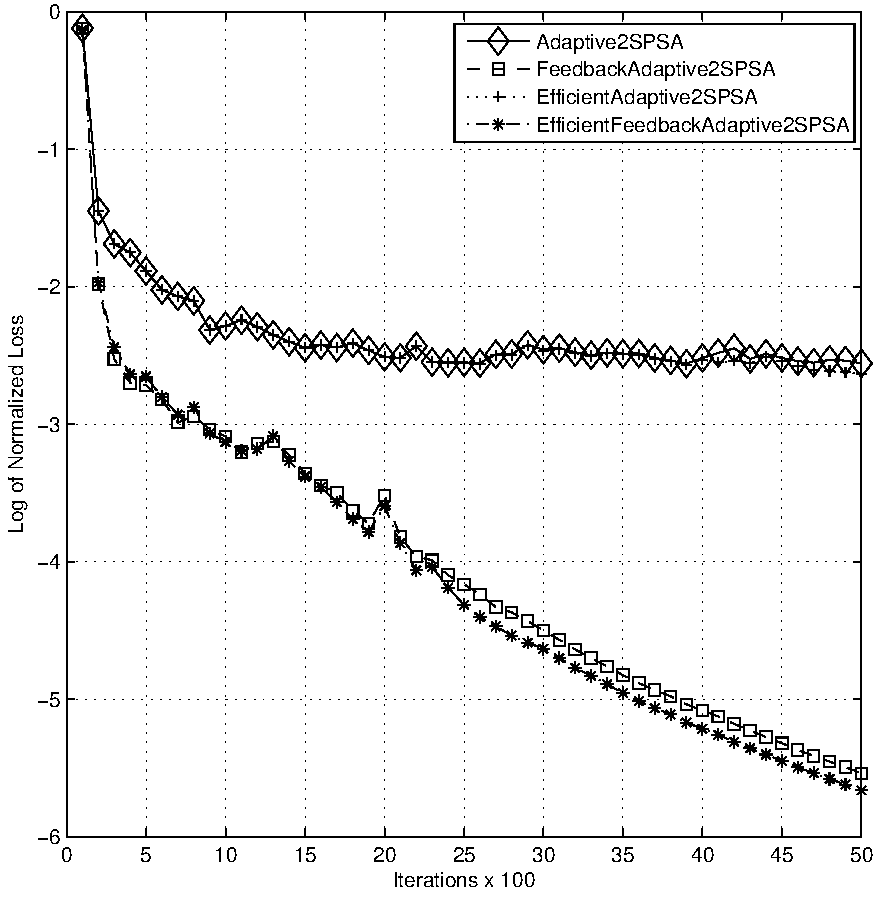
\includegraphics[width=1\columnwidth]{../res/NoNoise_normalized_loss_per_iteration.pdf}
  \caption{}
  \label{fig:normalizedloss}
\end{figure}

\begin{figure}[htbp]
	\centering
	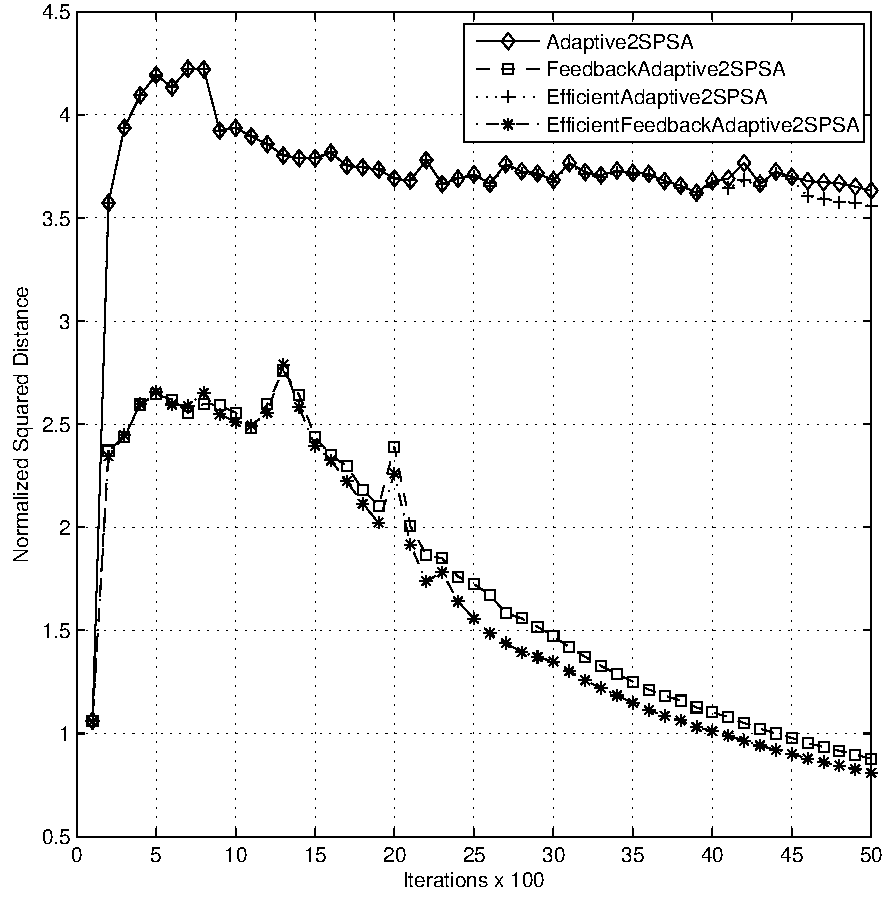
\includegraphics[width=1\columnwidth]{../res/NoNoise_normalized_squared_distance_per_iteration.pdf}
	\caption{}
	\label{fig:dist}
\end{figure}

\newcommand{\nruns}[0]{20\ }
To compare the original 2SPSA formulation, where the computation of $\ooH_k^{-1}
\bG_k(\htheta_k)$, with its more efficient
implementation, we first plot the normalized loss
$[L(\htheta_k)-L(\bm{\uptheta}^{*})]/[L(\htheta_0)-L(\bm{\uptheta}^{*})]$
against iteration $k$ averaging over \nruns simulation runs. Note that
both versions of the algorithms use the \textit{same} random seed and
are essentially performing the same iterations. Therefore we would expect
that the normalized loss sequences should be close to identical. This is evidenced by Figure~\ref{fig:normalizedloss}.

Figure~\ref{fig:dist} plots the Euclidean distance between
$\htheta_k$ and $\bm{\uptheta}^{*}$ against iteration $k$ averaging
over \nruns simulation runs.


Below is the table showing the time consumed in each step for $p=15$ case:
loss function evaluation, Hessian inverse update, pre-conditioning on
Hessian inverse, for A2SPSA and E2SPSA and their efficient implementations, efficient adaptive 2SPSA (EA2SPSA) and efficient enhanced 2SPSA (EE2SPSA).

\begin{table}[htbp]
	\centering
	\resizebox{\columnwidth}{!}{
		\begin{tabular}{l|ccccc|}
			\input{../res/timing_15.txt}
		\end{tabular}}
		\caption{Time Consumed in Each Procedure for $p=15$}
		\label{tab:time}
	\end{table}

Only consider the time consumed in the Hessian update recursion at each iteration. The second column in Table \ref{tab:time} shows that, the EA2SPSA only takes $81.82\%$ of the time taken in A2SPSA, and EE2SPSA only takes $77.31\%$ of that in E2SPSA.

The \textit{efficient} implementation can save more time with the original setup in Spall \cite{Spall2000} and \cite{Spall2009}, as the dimension $p$ goes up. To validate the relationship (\ref{eq:ratio1}-\ref{eq:ratio2}), we run the algorithms, using the same parameters tuned for dimension $p=15$, on different dimension $p=15,30,45,60,120$ and $240$.

\begin{table}[htbp]
	\centering
	\resizebox{\columnwidth}{!}{
		\begin{tabular}{l | c | c || r }
			
			 \hline
			 Dimension &  A2SPSA & EA2SPA & Ratio\\ \hline
			 15 & 0.363 & 0.297 & 0.8182\\
			 30 & 0.525 & 0.369 & 0.7029 \\
		 	 45 & 0.790 & 0.487 & 0.6165\\
			 60 & 1.094 & 0.654 & 0.5978 \\
			 120 & 3.575 & 1.844 & 0.5158 \\
			 240 &  1.881 & 0.942 & 0.5008\\
			 \hline
		\end{tabular}}
		\caption{Time Consumed in Hessian Update Procedure for Different Dimension  $p$
			\newline {\scriptsize  Ratio is time taken in A2SPSA over time taken in EA2SPSA}}
		\label{tab:timedifference1}
	\end{table}
	
	\begin{table}[htbp]
		\centering
		\resizebox{\columnwidth}{!}{
			\begin{tabular}{l | c | c || r }
				
				\hline
				Dimension &  E2SPSA & EE2SPA & Ratio\\ \hline
				15 & 0.432 & 0.334 & 0.7731\\
				30 & 0.565 & 0.398 & 0.7044 \\
				45 & 0.844 & 0.519 & 0.6149\\
				60 & 1.138 & 0.709 & 0.6230 \\
				120 & 3.517 & 1.899 & 0.5399 \\
				240 &  1.984 & 0.935 & 0.4713\\
				\hline
			\end{tabular}}
			\caption{Time Consumed in Hessian Update Procedure for Different Dimension  $p$
				\newline {\scriptsize  Ratio is time taken in E2SPSA over time taken in EE2SPSA}}
			\label{tab:timedifference2}
		\end{table}

From table \ref{tab:timedifference1}-\ref{tab:timedifference2}, we can envision the trend that the time consumed in the Hessian update procedure, where the sequential rank-one update \ref{eq:SequentialUpdate} makes a difference, is lesser in the efficient implementations than in the original setup in Spall~\cite{Spall2000} and \cite{Spall2009}. Though the ratio of time taken in efficient implementation over that in original setup is indeed decreasing as the dimension goes up, the ratio isn't decreasing as fast as (\ref{eq:ratio1}-\ref{eq:ratio2}) predict. The slower rate results from the efficiency of mldivide function (equivalently linsolve). The dimensions of our test matrices are far too small to manifest the asymptoptic $O(p^3)$ running time required by Gaussian-Jordan factorization in linsolve. Furthermore, MATLAB will typically be making use of parallel routines for computing the LU factorization. 

In short, this numerical example does show the superiority of the \textit{efficient} implementation of (\ref{eq:Transform}-\ref{eq:SequentialUpdate}), in terms of the running time and accuracy (though small as shown in Fig \ref{fig:dist}). The asymptotic ratio (\ref{eq:ratio1}-\ref{eq:ratio2}) hasn't been fully exploited in this small-dimensional example, though it is theoretically valid.


\section{Conclusion and Future Work} In this paper, we discuss
a coherent efficient implementation of four Newton-like SP algorithms:
adaptive 2SPSA, enhanced 2SPSA, adaptive 2SG, and enhanced 2SG. The
efficiency, in terms of both time taken and numerical accuracy, is
achieved by a unified sequential (rank-two) update using Woodbury
matrix identity. Particularly for the case of enhanced 2SG*, the
usage of symmetric Bernoulli perturbation sequence is required.

As discovered from practical experience, the time taken in the
stochastic optimization(minimization) problem is dominated by the
noisy function/gradient evaluation and the preconditioning part. We
are gathering ideas in speeding up the preconditioning step in the
algorithm, so as to magnify the contribution of this paper in
streamlining the Hessian inverse update.

\section*{Acknowledgment} The first author is sponsored by the
Defense Advanced Research Projects Agency (DARPA) under the Deep
Exploration and Filtering of Text (DEFT) Program (Agreement Number:
FA8750-13-2-001). Both the second and the third author receive
support from the Office of Naval Research (via Navy contract
N00024-13-D6400).

\begin{thebibliography}{1}
	
	\bibitem{Kiefer1952}
	Kiefer, J., and Wolfowitz, J. (1952). Stochastic estimation of the maximum of a regression function.\textit{ The Annals of Mathematical Statistics, 23(3)}, 462-466.
	
	\bibitem{Fabian1971}
	Fabian, V. (1971). Stochastic approximation, \textit{Optimizing Methods in Statistics}, J.S. Rustigi, Ed. New York: Academic Press, pp. 439-470.
	
	\bibitem{Ruppert1985}
	Ruppert, D. (1985). A Newton-Raphson version of the multivariate Robbins-Monro procedure. \textit{The Annals of Statistics}, 236-245.

\bibitem{Spall1992} Spall, J. C. (1992). Multivariate
  stochastic approximation using a simultaneous perturbation gradient
  approximation. \textit{Automatic Control, IEEE Transactions on},
  37(3), 332-341.

\bibitem{Spall2000} Spall, J. C. (2000). Adaptive
  stochastic approximation by the simultaneous perturbation
  method. \textit{Automatic Control, IEEE Transactions on}, 45(10),
  1839-1853.


\bibitem{Wang2011}
Wang, Q. (2011). Stochastic approximation for discrete optimization of noisy loss measurements. In \textit{2011 45th Annual Conference on Information Sciences and Systems} (pp. 1-4).  IEEE.



\bibitem{Spall2007}
Spall, J. C. (2007). Feedback and Weighting Mechanisms for Improving Jacobian Estimates in the Adaptive Simultaneous Perturbation Algorithm. In \textit{Information Sciences and Systems (CISS), 2007 41st Annual Conference on} (pp. 35-40). IEEE.


\bibitem{Spall2009} Spall, J. C. (2009). Feedback and
  weighting mechanisms for improving Jacobian estimates in the adaptive
  simultaneous perturbation algorithm. \textit{Automatic Control, IEEE
    Transactions on}, 54(6), 1216-1229.


\bibitem{Woodbury1950} Woodbury,
  M. A. (1950). Inverting Modified Matrices, Memorandum
  Rept. 42. \textit{Statistical Research Group, Princeton University,
    Princeton, NJ, 316}.

\remove
{
	\bibitem{Bar-Itzhack1998} Bar-Itzhack,
	I.Y. (1998). Matrix symmetrization. \textit{Journal of guidance,
		control, and dynamics}, 21(1), 178-179.
	}


\bibitem{Sadegh1998} Sadegh, P. and Spall,
  J. C. (1998). Optimal random perturbations for stochastic
  approximation using a simultaneous perturbation gradient
  approximation. \textit{Automatic Control, IEEE Transactions on}, 44,
  231-237.

\bibitem{Cao2011}
Cao, X. (2011, March). Effective perturbation distributions for small samples in simultaneous perturbation stochastic approximation. In \textit{Information Sciences and Systems (CISS), 2011 45th Annual Conference on} (pp. 1-5). IEEE.


\bibitem{Bhatnagar2012} Bhatnagar, S., Prasad,
  H. L. and Prashanth, L. A. (2013). \textit{Stochastic recursive
    algorithms for optimization: simultaneous perturbation methods},
  Springer.

\bibitem{Sylvester1867} Sylvester,
  J. J. (1867). LX. Thoughts on inverse orthogonal matrices,
  simultaneous signsuccessions, and tessellated pavements in two or more
  colours, with applications to Newton's rule, ornamental tile-work, and
  the theory of numbers. The London, Edinburgh, and Dublin Philosophical
  Magazine and Journal of Science, 34(232), pp. 461-475.

\bibitem{Bhatnagar2003}
Bhatnagar, S., Fu, M.C., Marcus, S.I. and Wang, I., 2003. Two-timescale simultaneous perturbation stochastic approximation using deterministic perturbation sequences. \textit{ACM Transactions on Modeling and Computer Simulation (TOMACS), 13(2)}, pp.180-209.

\end{thebibliography}
\end{document}

